\section{Propósito y protocolo temporal}
El análisis de varias ventanas permite examinar la disponibilidad y el significado de los indicadores conforme avanza una presentación. Esta fase de preparación de datos, correspondiente al segundo objetivo específico, construye una definición uniforme para los días 7, 14, 28, 42 y 56. El protocolo fue adoptado para esta versión por autorización del usuario y se registra en \texttt{decision\_temporal.json}; este registro no constituye una aprobación institucional adicional.

La unidad continúa siendo la inscripción de una persona en un módulo y una presentación de OULAD \cite{sdata2017171}. Para un corte $t$, se incluyen las inscripciones con fecha conocida de matrícula $r_i\leq t$, sin retiro administrativo $u_i\leq t$ y cuyo final de presentación $L_i$ es posterior al corte. Las fechas de retiro ausentes se interpretan como ausencia de retiro registrado. La etiqueta corresponde a
\[
Y_i(t)=\mathbf{1}\{t<u_i\leq L_i\}.
\]
Un retiro ocurrido exactamente en el día del corte se excluye de la población en riesgo. La observación abarca los días $0,1,\ldots,t$, incluidos ambos extremos; contiene $t+1$ días de calendario. Los antecedentes anteriores al inicio se calculan separadamente. Se supone disponibilidad al cierre del día de los registros de interacción y entrega, y disponibilidad previa del calendario de evaluación. Los archivos no permiten verificar retrasos de publicación ni revisiones históricas del calendario.

El horizonte llega hasta el final de cada presentación; su duración cambia entre cortes y cursos. Por tanto, la comparación no mantiene un horizonte de seguimiento de longitud fija. La etiqueta identifica retiro administrativo registrado y no demuestra su carácter voluntario ni equivale automáticamente a \textit{Withdrawn}. Las discordancias documentadas en la auditoría permanecen como limitación de la fuente.

\section{Población elegible y cambio de composición}
\Needspace{0.3\textheight}
\begingroup\small\setlength{\tabcolsep}{3pt}\renewcommand{\arraystretch}{1.16}
\begin{longtable}{>{\raggedright\arraybackslash}p{0.0870967741935484\linewidth}>{\raggedright\arraybackslash}p{0.23225806451612904\linewidth}>{\raggedright\arraybackslash}p{0.20322580645161292\linewidth}>{\raggedright\arraybackslash}p{0.22258064516129036\linewidth}>{\raggedright\arraybackslash}p{0.1548387096774194\linewidth}}
\caption{Población y evento propios de cada corte; el porcentaje usa inscripciones elegibles.}\label{multi02:poblacion}\\
\toprule
\textbf{Corte} & \textbf{Inscripciones} & \textbf{Personas} & \textbf{Retiros futuros} & \textbf{Porcentaje} \\
\midrule\endfirsthead
\toprule
\textbf{Corte} & \textbf{Inscripciones} & \textbf{Personas} & \textbf{Retiros futuros} & \textbf{Porcentaje} \\
\midrule\endhead
\bottomrule\endfoot
7 & 29\,076 & 26\,030 & 6\,632 & 22,81 \\*
14 & 28\,054 & 25\,220 & 5\,580 & 19,89 \\*
28 & 27\,515 & 24\,826 & 5\,012 & 18,22 \\*
42 & 27\,005 & 24\,491 & 4\,500 & 16,66 \\*
56 & 26\,506 & 24\,105 & 3\,998 & 15,08 \\*
\end{longtable}\endgroup
La disminución de la población refleja principalmente retiros ya ocurridos; también existen nuevas matrículas entre cortes. En consecuencia, las filas de cortes distintos no son observaciones independientes ni representan exactamente la misma población. La menor prevalencia posterior no demuestra una mejora educativa: se modifica la población en riesgo y se acorta el seguimiento. Los flujos secuenciales y los denominadores por módulo y presentación se conservan en las tablas exportadas.

\Needspace{0.3\textheight}
\begingroup\small\setlength{\tabcolsep}{3pt}\renewcommand{\arraystretch}{1.16}
\begin{longtable}{>{\raggedright\arraybackslash}p{0.12000000000000001\linewidth}>{\raggedright\arraybackslash}p{0.12000000000000001\linewidth}>{\raggedright\arraybackslash}p{0.24000000000000002\linewidth}>{\raggedright\arraybackslash}p{0.21000000000000002\linewidth}>{\raggedright\arraybackslash}p{0.21000000000000002\linewidth}}
\caption{Cambio de composición entre cortes consecutivos.}\label{multi02:transiciones}\\
\toprule
\textbf{Desde} & \textbf{Hasta} & \textbf{Comunes} & \textbf{Salen} & \textbf{Entran} \\
\midrule\endfirsthead
\toprule
\textbf{Desde} & \textbf{Hasta} & \textbf{Comunes} & \textbf{Salen} & \textbf{Entran} \\
\midrule\endhead
\bottomrule\endfoot
7 & 14 & 28\,019 & 1\,057 & 35 \\*
14 & 28 & 27\,477 & 577 & 38 \\*
28 & 42 & 27\,001 & 514 & 4 \\*
42 & 56 & 26\,503 & 502 & 3 \\*
\end{longtable}\endgroup

\begin{figure}[htbp]\centering
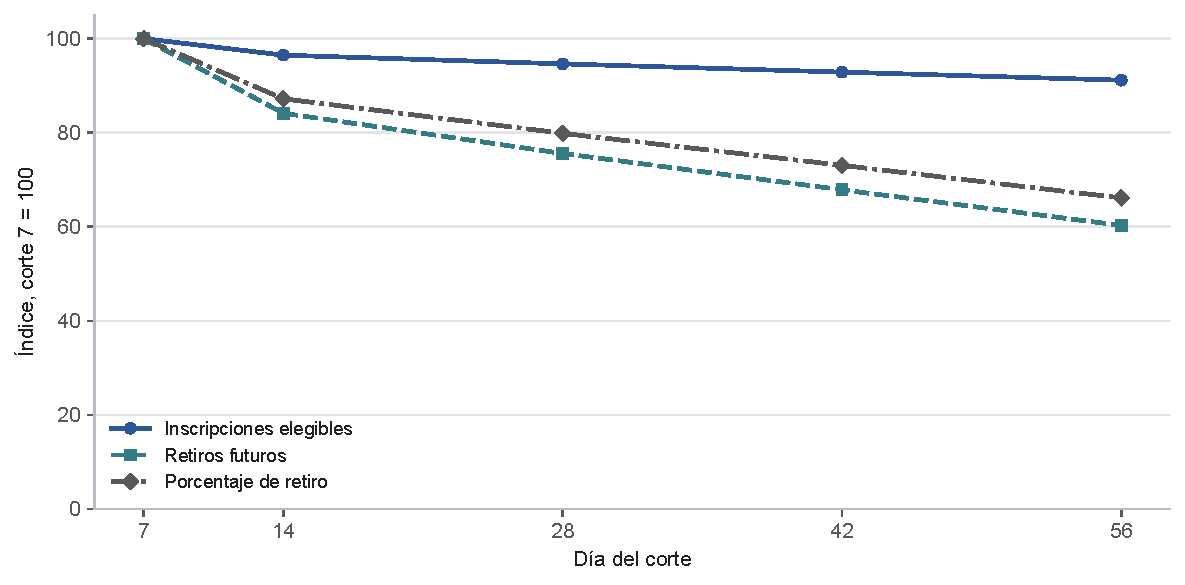
\includegraphics[width=.94\linewidth]{../figuras/02_poblacion_cortes.pdf}
\caption{Inscripciones elegibles, retiros futuros y prevalencia: índice con corte 7 igual a 100. Las líneas unen poblaciones distintas; no son trayectorias de una cohorte.}\label{multi02:figpoblacion}\end{figure}
\section{Construcción y disponibilidad de indicadores}
La actividad se resume mediante volumen de clics, días activos, frecuencia relativa, recencia y variabilidad de los totales diarios. Un día activo contiene al menos un clic; la proporción de días activos usa $t+1$ como denominador. Esta normalización facilita una lectura temporal, pero no corrige la menor exposición de las matrículas posteriores al inicio. Se exporta adicionalmente el número de días matriculados dentro de la ventana para identificar esta condición. El número de filas VLE no se denomina número de sesiones.

La recencia es la diferencia entre el corte y el último día activo; se conserva ausente cuando no existe actividad en la ventana. El coeficiente de variación emplea la desviación estándar muestral de los totales diarios, incluidos los ceros, dividida por su media. También se cuentan semanas completas desde el día 0 y se omite el bloque final incompleto. Estos indicadores describen conductas observables; los clics no constituyen una medición directa de motivación.

La tendencia compara bloques contiguos de igual longitud que terminan en el corte. Para $s=7$ o $s=14$, se calcula
\[
T_{i,s}(t)=\log\!\left(\frac{1+\sum_{d=t-s+1}^{t}c_{id}}
{1+\sum_{d=t-2s+1}^{t-s}c_{id}}\right).
\]
El término 1 permite razones finitas cuando un solo bloque tiene cero clics. Si ambos bloques son cero, la tendencia se conserva ausente; tampoco se calcula cuando existen menos de $2s$ días de historia. De este modo, la tendencia de siete días no está disponible en el corte 7 y la de catorce días solo se calcula desde el corte 28.

La inactividad acumulada y la ausencia de clics en los últimos 7, 14 o 28 días se conservan como indicadores complementarios. Una ventana reciente sin historia suficiente se representa como no observable, no como actividad ni como inactividad. Ninguna de estas banderas sustituye la etiqueta administrativa; su interpretación depende del calendario y de las oportunidades de participación.

Las entregas incluyen evaluaciones distintas de \textit{Exam}, sin reconocimiento de otra presentación (\textit{banked}), observadas entre 0 y $t$. Se distinguen las evaluaciones programadas hasta el corte y cuántas de ellas ya fueron entregadas; estas últimas pueden haberse entregado antes del inicio. La proporción entregada no mide puntualidad y queda ausente cuando no hay evaluaciones programadas. Los puntajes y su disponibilidad se conservan únicamente para auditoría, porque la fecha de entrega no acredita la fecha de publicación de la nota.

\Needspace{0.3\textheight}
\begingroup\small\setlength{\tabcolsep}{3pt}\renewcommand{\arraystretch}{1.16}
\begin{longtable}{>{\raggedright\arraybackslash}p{0.07422680412371135\linewidth}>{\raggedright\arraybackslash}p{0.18556701030927839\linewidth}>{\raggedright\arraybackslash}p{0.25979381443298977\linewidth}>{\raggedright\arraybackslash}p{0.17628865979381445\linewidth}>{\raggedright\arraybackslash}p{0.2041237113402062\linewidth}}
\caption{Disponibilidad y exposición en la población elegible; conteos de inscripciones.}\label{multi02:disponibilidad}\\
\toprule
\textbf{Corte} & \textbf{Sin actividad} & \textbf{Sin evaluación programada} & \textbf{Con entregas} & \textbf{Matrícula después de 0} \\
\midrule\endfirsthead
\toprule
\textbf{Corte} & \textbf{Sin actividad} & \textbf{Sin evaluación programada} & \textbf{Con entregas} & \textbf{Matrícula después de 0} \\
\midrule\endhead
\bottomrule\endfoot
7 & 5\,316 & 29\,076 & 772 & 140 \\*
14 & 2\,551 & 26\,765 & 3\,226 & 173 \\*
28 & 1\,203 & 4\,988 & 19\,849 & 208 \\*
42 & 918 & 2\,426 & 22\,276 & 210 \\*
56 & 765 & 2\,407 & 22\,812 & 212 \\*
\end{longtable}\endgroup
En el corte 7 ninguna inscripción tiene evaluaciones con vencimiento entre 0 y 7, aunque 772 ya presentan entregas. Por ello, ausencia de entregas y falta de cumplimiento no son equivalentes. En el corte 28 persisten 4\,988 inscripciones sin evaluación programada y en el corte 56 son 2\,407; la ampliación de la ventana no elimina toda la heterogeneidad del calendario.

\section{Enlace con la versión anterior y productos}
La versión anterior del corte 28 observaba actividad hasta el día 27. La versión actual incorpora también el día 28 y mantiene las 27\,515 inscripciones elegibles. Esta modificación explica cambios de cifras sin atribuirlos a alteraciones de las fuentes.

\Needspace{0.3\textheight}
\begingroup\small\setlength{\tabcolsep}{3pt}\renewcommand{\arraystretch}{1.16}
\begin{longtable}{>{\raggedright\arraybackslash}p{0.23\linewidth}>{\raggedright\arraybackslash}p{0.23\linewidth}>{\raggedright\arraybackslash}p{0.23\linewidth}>{\raggedright\arraybackslash}p{0.25\linewidth}}
\caption{Efecto de incluir el día 28 en las mismas inscripciones.}\label{multi02:enlace}\\
\toprule
\textbf{Indicador} & \textbf{Anterior} & \textbf{Actual} & \textbf{Inscripciones con cambio} \\
\midrule\endfirsthead
\toprule
\textbf{Indicador} & \textbf{Anterior} & \textbf{Actual} & \textbf{Inscripciones con cambio} \\
\midrule\endhead
\bottomrule\endfoot
Clics & 7\,603\,586 & 7\,766\,285 & 7\,993 \\*
Entregas & 22\,870 & 23\,136 & 263 \\*
\end{longtable}\endgroup
Se exportan conjuntos separados de datos auditables, predictores y etiquetas para cada corte; las claves se conservan para vincularlos, sin convertir el identificador de estudiante en predictor. El diccionario documenta 26 indicadores candidatos y separa las variables de contexto. La tabla apilada tiene una fila por inscripción y corte, no por persona. La intersección de los cinco conjuntos contiene 26\,429 inscripciones y se utiliza únicamente para una sensibilidad retrospectiva.

Los productos permiten continuar con un protocolo predictivo común. El ajuste de imputación, escalado, selección y cualquier remuestreo deberá realizarse dentro del entrenamiento de cada partición \cite{revsklearnpitfalls}. Esta fase no entrenó clasificadores, no seleccionó una ventana óptima y no ofrece evidencia de desempeño fuera de muestra. Antes de modelar deberán fijarse la generalización buscada y la separación por personas o presentaciones; una persona presente en varios cortes no debe contaminar conjuntos de entrenamiento y evaluación.


\section{Notación y definición de la tarea temporal}
El día 0 es el inicio de la presentación; las fechas negativas son anteriores a ese origen. La unidad $i$ es la terna de persona, módulo y presentación. Para cada corte $t$, $n_t=t+1$ es la longitud inclusiva del calendario observado, $r_i$ es la fecha de matrícula, $u_i$ la fecha de retiro cuando existe y $L_i$ el final según la convención operativa basada en la longitud registrada de la presentación. La ventana principal es $\{0,\ldots,t\}$ y el horizonte futuro es $(t,L_i]$; los antecedentes preinicio se construyen separadamente.
\Needspace{0.42\textheight}
\begingroup\small\setlength{\tabcolsep}{3pt}\renewcommand{\arraystretch}{1.16}
\begin{longtable}{>{\raggedright\arraybackslash}p{0.27\linewidth}>{\raggedright\arraybackslash}p{0.67\linewidth}}
\caption{Guía de símbolos; los índices de modelos se definen localmente en su formulación.}\label{corr:simbolos}\\
\toprule
\textbf{Símbolo en las ecuaciones} & \textbf{Significado} \\
\midrule\endfirsthead
\toprule
\textbf{Símbolo en las ecuaciones} & \textbf{Significado} \\
\midrule\endhead
\bottomrule\endfoot
$i$ & Inscripción: persona, módulo y presentación \\*
$d,t$ & Día relativo al inicio y corte de predicción \\*
$n_t$ & Número de días observados: t+1 \\*
$r_i,u_i,L_i$ & Matrícula, retiro y final de presentación \\*
$c_{id},A_i(t)$ & Clics diarios y conjunto de días activos \\*
$V_i,k_i,q_i,m_i$ & Volumen, días activos, proporción activa e intensidad \\*
$N(t),E(t),\pi(t)$ & Inscripciones elegibles, eventos futuros y prevalencia \\*
$Y_i(t)$ & Evento binario posterior al corte y hasta el final \\*
$p(\mathbf{x}),\tau$ & Probabilidad condicional y umbral de clasificación \\*
$\phi_j$ & Contribución de Shapley en una escala y referencia fijadas \\*
\end{longtable}\endgroup
\begin{align}
\mathcal E(t)&=\{i:r_i\text{ conocida},\ r_i\le t,\ (u_i\text{ ausente o }u_i>t),\ L_i>t\},\label{corr:elegibilidad}\\
N(t)&=|\mathcal E(t)|,\quad Y_i(t)=\mathbf 1\{t<u_i\le L_i\},\label{corr:evento}\\
E(t)&=\sum_{i\in\mathcal E(t)}Y_i(t),\qquad \pi(t)=E(t)/N(t).\label{corr:prevalencia}
\end{align}
La función $\mathbf 1$ vale uno cuando se cumple su condición y cero en otro caso; en particular, una fecha ausente no genera evento. Las barras $|\cdot|$ representan el número de elementos de un conjunto. La clase negativa significa ausencia de retiro registrado dentro del horizonte, no éxito académico ni permanencia acreditada. Los retiros del día del corte ya ocurrieron y quedan excluidos. El horizonte disminuye con $t$ y varía entre presentaciones; la comparación mantiene reglas, no una misma duración de seguimiento.

Sean $c_{id}$ los clics totales del día $d$ y $A_i(t)=\{d\in[0,t]:c_{id}>0\}$. El volumen, los días activos, la proporción activa y la intensidad se definen como
\begin{equation}
V_i(t)=\sum_{d=0}^t c_{id},\quad k_i(t)=|A_i(t)|,\quad q_i(t)=\frac{k_i(t)}{n_t},\quad m_i(t)=\frac{V_i(t)}{k_i(t)}\quad(k_i(t)>0).\label{corr:actividad}
\end{equation}
La recencia es $t-\max A_i(t)$ y su versión relativa divide por $n_t$; ambas permanecen ausentes cuando no hay actividad. El CV de intensidad activa es la desviación estándar muestral de los clics en $A_i(t)$ dividida por su media; requiere $k_i(t)\ge2$. El CV de calendario conserva los ceros. Para abreviar, con $n=n_t$, $k=k_i(t)$ y $q=k/n$,
\begin{equation}
CV_{cal}^{2}=\frac{n}{n-1}\left[\frac{1-q}{q}+\frac{k-1}{kq}CV_{act}^{2}\right],\qquad k\ge2.\label{corr:identidadcv}
\end{equation}
La identidad se obtiene al descomponer la suma de cuadrados de los días activos como $(k-1)s_{act}^{2}+k m^{2}$ y usar la media de calendario $qm$. El primer término recoge la inactividad y el segundo la dispersión de intensidad; solo con intensidad constante se reduce a una función de $q$. Ningún CV se presenta como evidencia independiente de la frecuencia por el solo hecho de tener otro nombre.

El sumando 1 de la tendencia permite cocientes finitos con un bloque nulo. Se trata de un suavizado: intercambiar los bloques invierte exactamente el signo, pero escalar los conteos no conserva necesariamente el valor. Ambos bloques nulos se representan como no observables. La tendencia de siete días requiere $t\ge13$ y la de catorce $t\ge27$; 14 y 28 son los primeros cortes elegidos que cumplen esas condiciones, no los primeros matemáticamente posibles.

\section{Selección de indicadores y diferencias respecto del anteproyecto}
El conteo \texttt{n\_registros\_vle} mide filas originales por inscripción en $[0,t]$, sin identificar sesiones. Su granularidad y sus repeticiones no están explicadas por la fuente. Se conserva para auditoría y se retira del conjunto predictivo principal. Esta decisión evita atribuir a una frecuencia de registro un significado educativo que no ha sido verificado; el VIF documentado aporta una razón adicional de redundancia, pero no es por sí solo una regla universal de exclusión.

La diversidad de recursos y tipos de actividad no se construye en esta versión. El conjunto se delimita a volumen, continuidad, recencia, variación temporal y participación evaluativa, conservando el diseño de indicadores examinado y añadiendo la comparación entre ambos CV. Esta delimitación no demuestra falta de utilidad de diversidad: su evaluación requeriría integrar el catálogo de recursos y considerar oportunidades diferentes entre módulos. La familia se mantiene en el marco como posibilidad derivable, con esta exclusión explícita de la implementación actual.

La actividad A3.1 del anteproyecto interpreta la fecha como retiro voluntario y propone explorar abandono implícito. Los archivos permiten ubicar la baja pero no demostrar su motivo; por ello, se adopta el retiro registrado futuro y se mantiene la inactividad como indicador complementario. La predicción de inactividad en un periodo futuro sería otra tarea, no necesariamente circular; no se adopta como segunda etiqueta en esta versión. A2.5 contempla puntajes, que se conservan solo para auditoría porque falta su fecha de publicación. Estas diferencias y la restricción de población al corte deben ratificarse académicamente; la autorización de trabajo no constituye un acta institucional.

La rejilla se adoptó antes de comparar modelos y conserva hitos de una, dos, cuatro, seis y ocho semanas. Las presentaciones duran entre 234 y 269 días; el corte 56 cae dentro del primer cuarto. La computabilidad y el calendario describen la pertinencia de la rejilla, pero no demuestran que sea óptima ni que se haya seleccionado sin conocimiento previo del desenlace. Los datos de calendario publicados permiten examinar la disponibilidad académica, presente ya al día 14.
\section{Cascadas completas de elegibilidad}
La Tabla~\ref{corr:flujos} publica cada filtro y sus denominadores. Las exclusiones son secuenciales, no categorías superpuestas. Después del filtro de matrícula quedan 2\,643 retiros preinicio; los 35 restantes de la fuente completa ya fueron excluidos por matrícula.
\Needspace{0.2\textheight}
\begingroup\small\setlength{\tabcolsep}{3pt}\renewcommand{\arraystretch}{1.16}
\begin{longtable}{>{\raggedright\arraybackslash}p{0.0670212765957447\linewidth}>{\raggedright\arraybackslash}p{0.32553191489361705\linewidth}>{\raggedright\arraybackslash}p{0.19148936170212766\linewidth}>{\raggedright\arraybackslash}p{0.1723404255319149\linewidth}>{\raggedright\arraybackslash}p{0.14361702127659576\linewidth}}
\caption{Flujo secuencial en cada corte; las exclusiones corresponden a la etapa indicada.}\label{corr:flujos}\\
\toprule
\textbf{Corte} & \textbf{Etapa} & \textbf{Inscripciones} & \textbf{Personas} & \textbf{Excluidas} \\
\midrule\endfirsthead
\toprule
\textbf{Corte} & \textbf{Etapa} & \textbf{Inscripciones} & \textbf{Personas} & \textbf{Excluidas} \\
\midrule\endhead
\bottomrule\endfoot
7 & Fuente & 32\,593 & 28\,785 & 0 \\
7 & Matrícula conocida & 32\,548 & 28\,755 & 45 \\
7 & Matriculada al corte & 32\,455 & 28\,691 & 93 \\
7 & Sin retiro hasta corte & 29\,076 & 26\,030 & 3\,379 \\
7 & Final posterior al corte & 29\,076 & 26\,030 & 0 \\
14 & Fuente & 32\,593 & 28\,785 & 0 \\
14 & Matrícula conocida & 32\,548 & 28\,755 & 45 \\
14 & Matriculada al corte & 32\,490 & 28\,715 & 58 \\
14 & Sin retiro hasta corte & 28\,054 & 25\,220 & 4\,436 \\
14 & Final posterior al corte & 28\,054 & 25\,220 & 0 \\
28 & Fuente & 32\,593 & 28\,785 & 0 \\
28 & Matrícula conocida & 32\,548 & 28\,755 & 45 \\
28 & Matriculada al corte & 32\,532 & 28\,748 & 16 \\
28 & Sin retiro hasta corte & 27\,515 & 24\,826 & 5\,017 \\
28 & Final posterior al corte & 27\,515 & 24\,826 & 0 \\
42 & Fuente & 32\,593 & 28\,785 & 0 \\
42 & Matrícula conocida & 32\,548 & 28\,755 & 45 \\
42 & Matriculada al corte & 32\,536 & 28\,750 & 12 \\
42 & Sin retiro hasta corte & 27\,005 & 24\,491 & 5\,531 \\
42 & Final posterior al corte & 27\,005 & 24\,491 & 0 \\
56 & Fuente & 32\,593 & 28\,785 & 0 \\
56 & Matrícula conocida & 32\,548 & 28\,755 & 45 \\
56 & Matriculada al corte & 32\,539 & 28\,753 & 9 \\
56 & Sin retiro hasta corte & 26\,506 & 24\,105 & 6\,033 \\
56 & Final posterior al corte & 26\,506 & 24\,105 & 0 \\
\end{longtable}\endgroup
\section{Disponibilidad y calendario}
El primer vencimiento continuo varía entre los días 12 y 61 según la presentación. En el corte 7 hay entregas anticipadas aunque no haya vencimientos. La falta de oportunidad no equivale a incumplimiento.

\begin{figure}[H]\centering
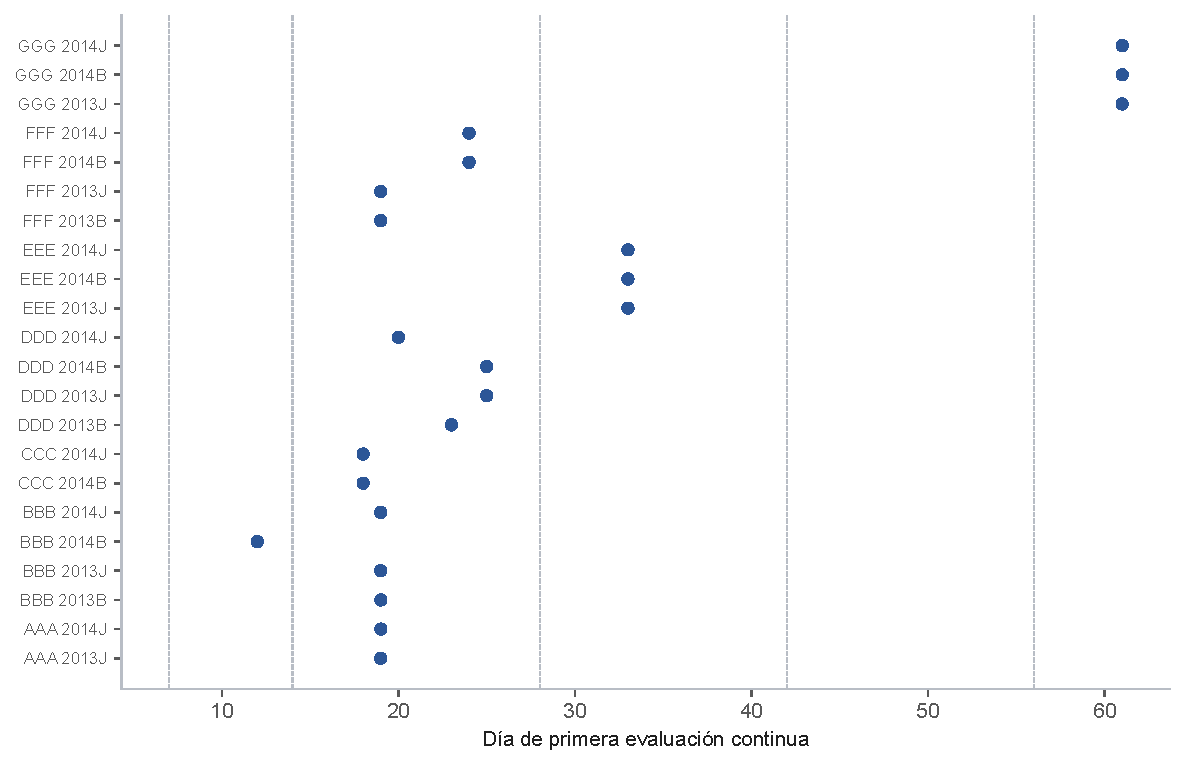
\includegraphics[width=.94\linewidth]{../figuras/02_calendario_evaluaciones.pdf}
\caption{Primer vencimiento no Exam por módulo y presentación.}\label{corr:calendario}\end{figure}

\begin{figure}[H]\centering
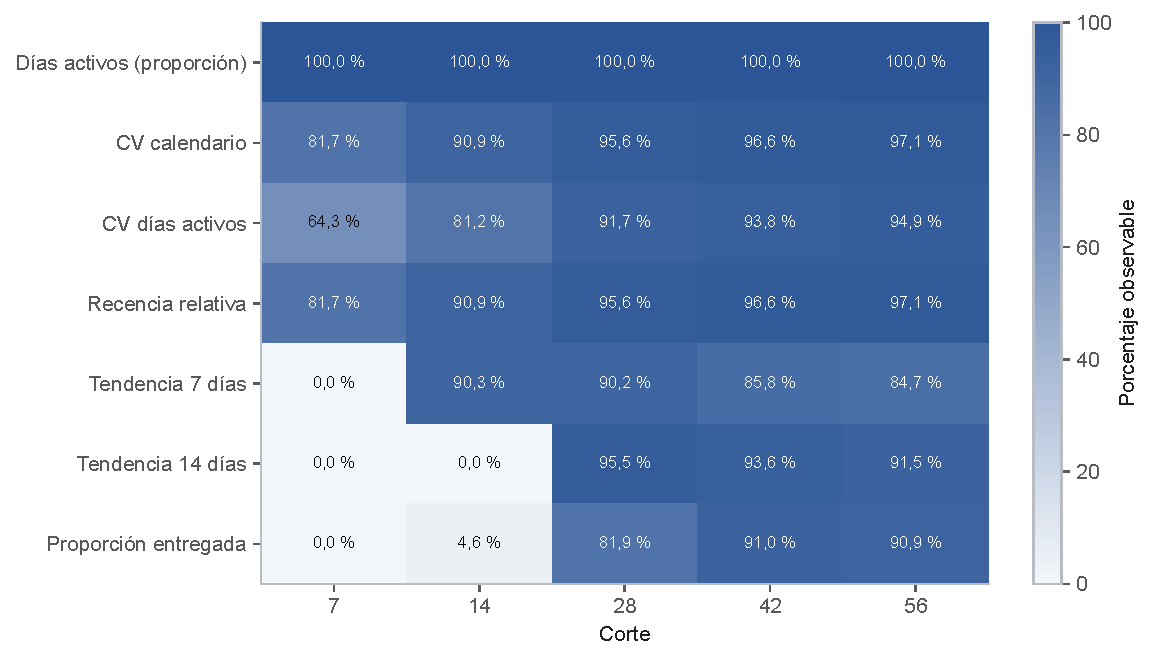
\includegraphics[width=.94\linewidth]{../figuras/02_disponibilidad_indicadores.pdf}
\caption{Observabilidad de cada indicador; porcentaje de inscripciones elegibles en cada corte.}\label{corr:observabilidad}\end{figure}
\section{Diccionario reconciliado de indicadores}
Se documentan 26 candidatos, incluidos ambos CV; no se han seleccionado variables mediante desempeño predictivo. El conteo de filas aparece únicamente como auditoría. Los identificadores, el contexto y los desenlaces permanecen separados.
\Needspace{0.2\textheight}
\begingroup\small\setlength{\tabcolsep}{3pt}\renewcommand{\arraystretch}{1.16}
\begin{longtable}{>{\raggedright\arraybackslash}p{0.29\linewidth}>{\raggedright\arraybackslash}p{0.43\linewidth}>{\raggedright\arraybackslash}p{0.22\linewidth}}
\caption{Diccionario de candidatos y conteo de filas de auditoría; nombres idénticos al código.}\label{corr:diccionario}\\
\toprule
\textbf{Variable} & \textbf{Definición} & \textbf{Dominio y ausencia} \\
\midrule\endfirsthead
\toprule
\textbf{Variable} & \textbf{Definición} & \textbf{Dominio y ausencia} \\
\midrule\endhead
\bottomrule\endfoot
total\_\allowbreak{}clics & Suma de clics en 0..t & entero >= 0 \\
dias\_\allowbreak{}activos & Días con clics en 0..t & 0..t+1 \\
proporcion\_\allowbreak{}dias\_\allowbreak{}activos & dias\_\allowbreak{}activos/(t+1); calendario completo, no exposición individual & [0,1] \\
n\_\allowbreak{}registros\_\allowbreak{}vle & Filas de la fuente en 0..t; no son sesiones & entero >= 0 \\
promedio\_\allowbreak{}clics\_\allowbreak{}por\_\allowbreak{}dia\_\allowbreak{}activo & total\_\allowbreak{}clics/dias\_\allowbreak{}activos & NaN sin actividad \\
coef\_\allowbreak{}variacion\_\allowbreak{}clics & SD muestral de t+1 totales diarios / media; incluye ceros & NaN sin actividad \\
cv\_\allowbreak{}intensidad\_\allowbreak{}activa & SD muestral / media de clics solo en días activos; intensidad condicional & NaN si días activos < 2 \\
dias\_\allowbreak{}desde\_\allowbreak{}ultima\_\allowbreak{}interaccion & t - último día activo dentro de 0..t & NaN sin actividad \\
recencia\_\allowbreak{}relativa & Recencia/(t+1) & NaN sin actividad \\
semanas\_\allowbreak{}completas\_\allowbreak{}activas & Bloques completos de 7 días desde 0 con actividad; omite bloque final parcial & 0..floor((t+1)/7) \\
proporcion\_\allowbreak{}semanas\_\allowbreak{}completas\_\allowbreak{}activas & Semanas completas activas / floor((t+1)/7) & [0,1] \\
clics\_\allowbreak{}pre\_\allowbreak{}inicio & Clics con fecha < 0 & entero >= 0 \\
sin\_\allowbreak{}actividad\_\allowbreak{}acumulada & 1 si total\_\allowbreak{}clics=0 & 0/1 \\
sin\_\allowbreak{}actividad\_\allowbreak{}ultimos\_\allowbreak{}7d & 1 si no hay clics en t-6..t & NaN con menos de 7 días observados \\
sin\_\allowbreak{}actividad\_\allowbreak{}ultimos\_\allowbreak{}14d & 1 si no hay clics en t-13..t & NaN con menos de 14 días observados \\
sin\_\allowbreak{}actividad\_\allowbreak{}ultimos\_\allowbreak{}28d & 1 si no hay clics en t-27..t & NaN con menos de 28 días observados \\
clics\_\allowbreak{}ultimos\_\allowbreak{}7d & Clics en t-6..t & NaN si observación < 7 días \\
clics\_\allowbreak{}7d\_\allowbreak{}previos & Clics en t-13..t-7 & NaN si observación < 14 días \\
log\_\allowbreak{}ratio\_\allowbreak{}7d & ln((clics últimos 7d+1)/(clics 7d previos+1)) & NaN con historia <14 días o cero en ambos bloques \\
log\_\allowbreak{}ratio\_\allowbreak{}14d & Razón logarítmica suavizada entre últimos dos bloques de 14 días & NaN con historia <28 días o cero en ambos bloques \\
n\_\allowbreak{}evaluaciones\_\allowbreak{}entregadas & Evaluaciones no Exam ni banked entregadas en 0..t & entero >= 0 \\
n\_\allowbreak{}entregas\_\allowbreak{}pre\_\allowbreak{}inicio & Entregas no Exam ni banked anteriores a 0 & entero >= 0 \\
n\_\allowbreak{}evaluaciones\_\allowbreak{}programadas & Evaluaciones no Exam con fecha de calendario en 0..t & entero >= 0 \\
n\_\allowbreak{}programadas\_\allowbreak{}entregadas\_\allowbreak{}al\_\allowbreak{}corte & Evaluaciones programadas en 0..t entregadas hasta t, sin banked & 0..n programadas \\
proporcion\_\allowbreak{}programadas\_\allowbreak{}entregadas & Entregadas programadas / programadas; no mide puntualidad & NaN si no hay programadas \\
sin\_\allowbreak{}evaluacion\_\allowbreak{}programada & 1 si no existen evaluaciones programadas en 0..t & 0/1 \\
sin\_\allowbreak{}entregas\_\allowbreak{}acumuladas & 1 si no hay entregas no Exam ni banked en 0..t; no implica incumplimiento & 0/1 \\
\end{longtable}\endgroup
